\section{Geocodierung in Google Fusion Tables}
\label{gft-geocoding}
Ein grosser Vorteil der Google Fusion Tables ist die automatische 
\gls{Geocodierung} von Standortdaten. Sobald eine neue Zeile via Web-GUI zu einer Tabelle hinzugefügt wird, werden alle Zellen vom Typ \emph{Location} einem eindeutigen Standort auf der Karte zugewiesen. Ist dies nicht möglich, da beispielsweise eine Adresse in mehreren Orten vorkommen kann, wird die Zelle nicht geocodiert und der Text wird gelb hinterlegt. In solchen Fällen hat man die Möglichkeit den zugehörigen Ort manuell mit Hilfe einer Karte zu wählen.

\begin{figure}[!ht]
	\centering
	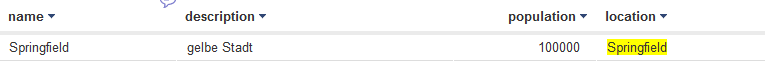
\includegraphics[width=\textwidth]{images/einfuehrung/geocoding_failed}
	\caption{Geocodierung für Ort Springfield fehlgeschlagen}
	\label{geocoding_failed}
\end{figure}

Die geocodierten Standorte werden als Metadaten in der Tabelle hinterlegt. Leider sind diese Daten über das SQL \gls{API} nicht selektierbar. Möchte man die erhaltenen Daten auf der Karte positionieren, so muss man für jede Zeile die \gls{Geocodierung} manuell vornehmen, was sich negativ auf die Ladezeit der Karte auswirkt.

\subsection{Geocoding-Dienste}
Es gibt verschiedene Dienste, welche eine solche \gls{Geocodierung} von Standortdaten anbieten. Die meisten davon haben aber eine Begrenzung der möglichen Anfragen pro Tag.

\begin{table}[H]
\centering
\begin{tabular}{|p{0.4\threecelltabwidth}|p{0.14\threecelltabwidth}|p{0.46\threecelltabwidth}|}
\hline 
\textbf{Anbieter} & \textbf{Anfragen pro Tag} & \textbf{URL} \\ 
\hline 
Google Maps Geocoding \gls{API} & 2500 & \url{https://developers.google.com/maps/documentation/geocoding/?hl=de} \\ 
\hline 
Yahoo! PlaceFinder \gls{API} & 50000 & \url{http://developer.yahoo.com/geo/placefinder/} \\ 
\hline 
MapQuest Geocoding \gls{API} & keine Begrenzung & \url{http://developer.mapquest.com/web/products/dev-services/geocoding-ws} \\ 
\hline 
\end{tabular}
\caption{Geocoding Limitierungen}
\end{table} 

\subsection{Geocoding von neuen Datensätzen}
\label{geocodierung-bug}
Ein grosses Problem stellt sich darin, dass neue Datensätze, welche über das SQL \gls{API} eingefügt wurden, nicht automatisch geocodiert werden. Dies führt dazu, dass diese Daten von Abfragen, welche eine ortsbezogene Einschränkung beinhalten (siehe Abschnitt \ref{sqlapi-spatialqueries}), nicht zurückgeliefert werden.

Eine \gls{Geocodierung} dieser Daten kann nur manuell über das Fusion Tables Web-GUI gestartet werden.